
% https://docs.google.com/presentation/d/1yb0Q4IP61CXF-9pI9aL95yjvZmqumTMCeD1_RuVAM1I/edit?slide=id.g3676c470f8c_0_0#slide=id.g3676c470f8c_0_0

\begin{figure}
    \centering
    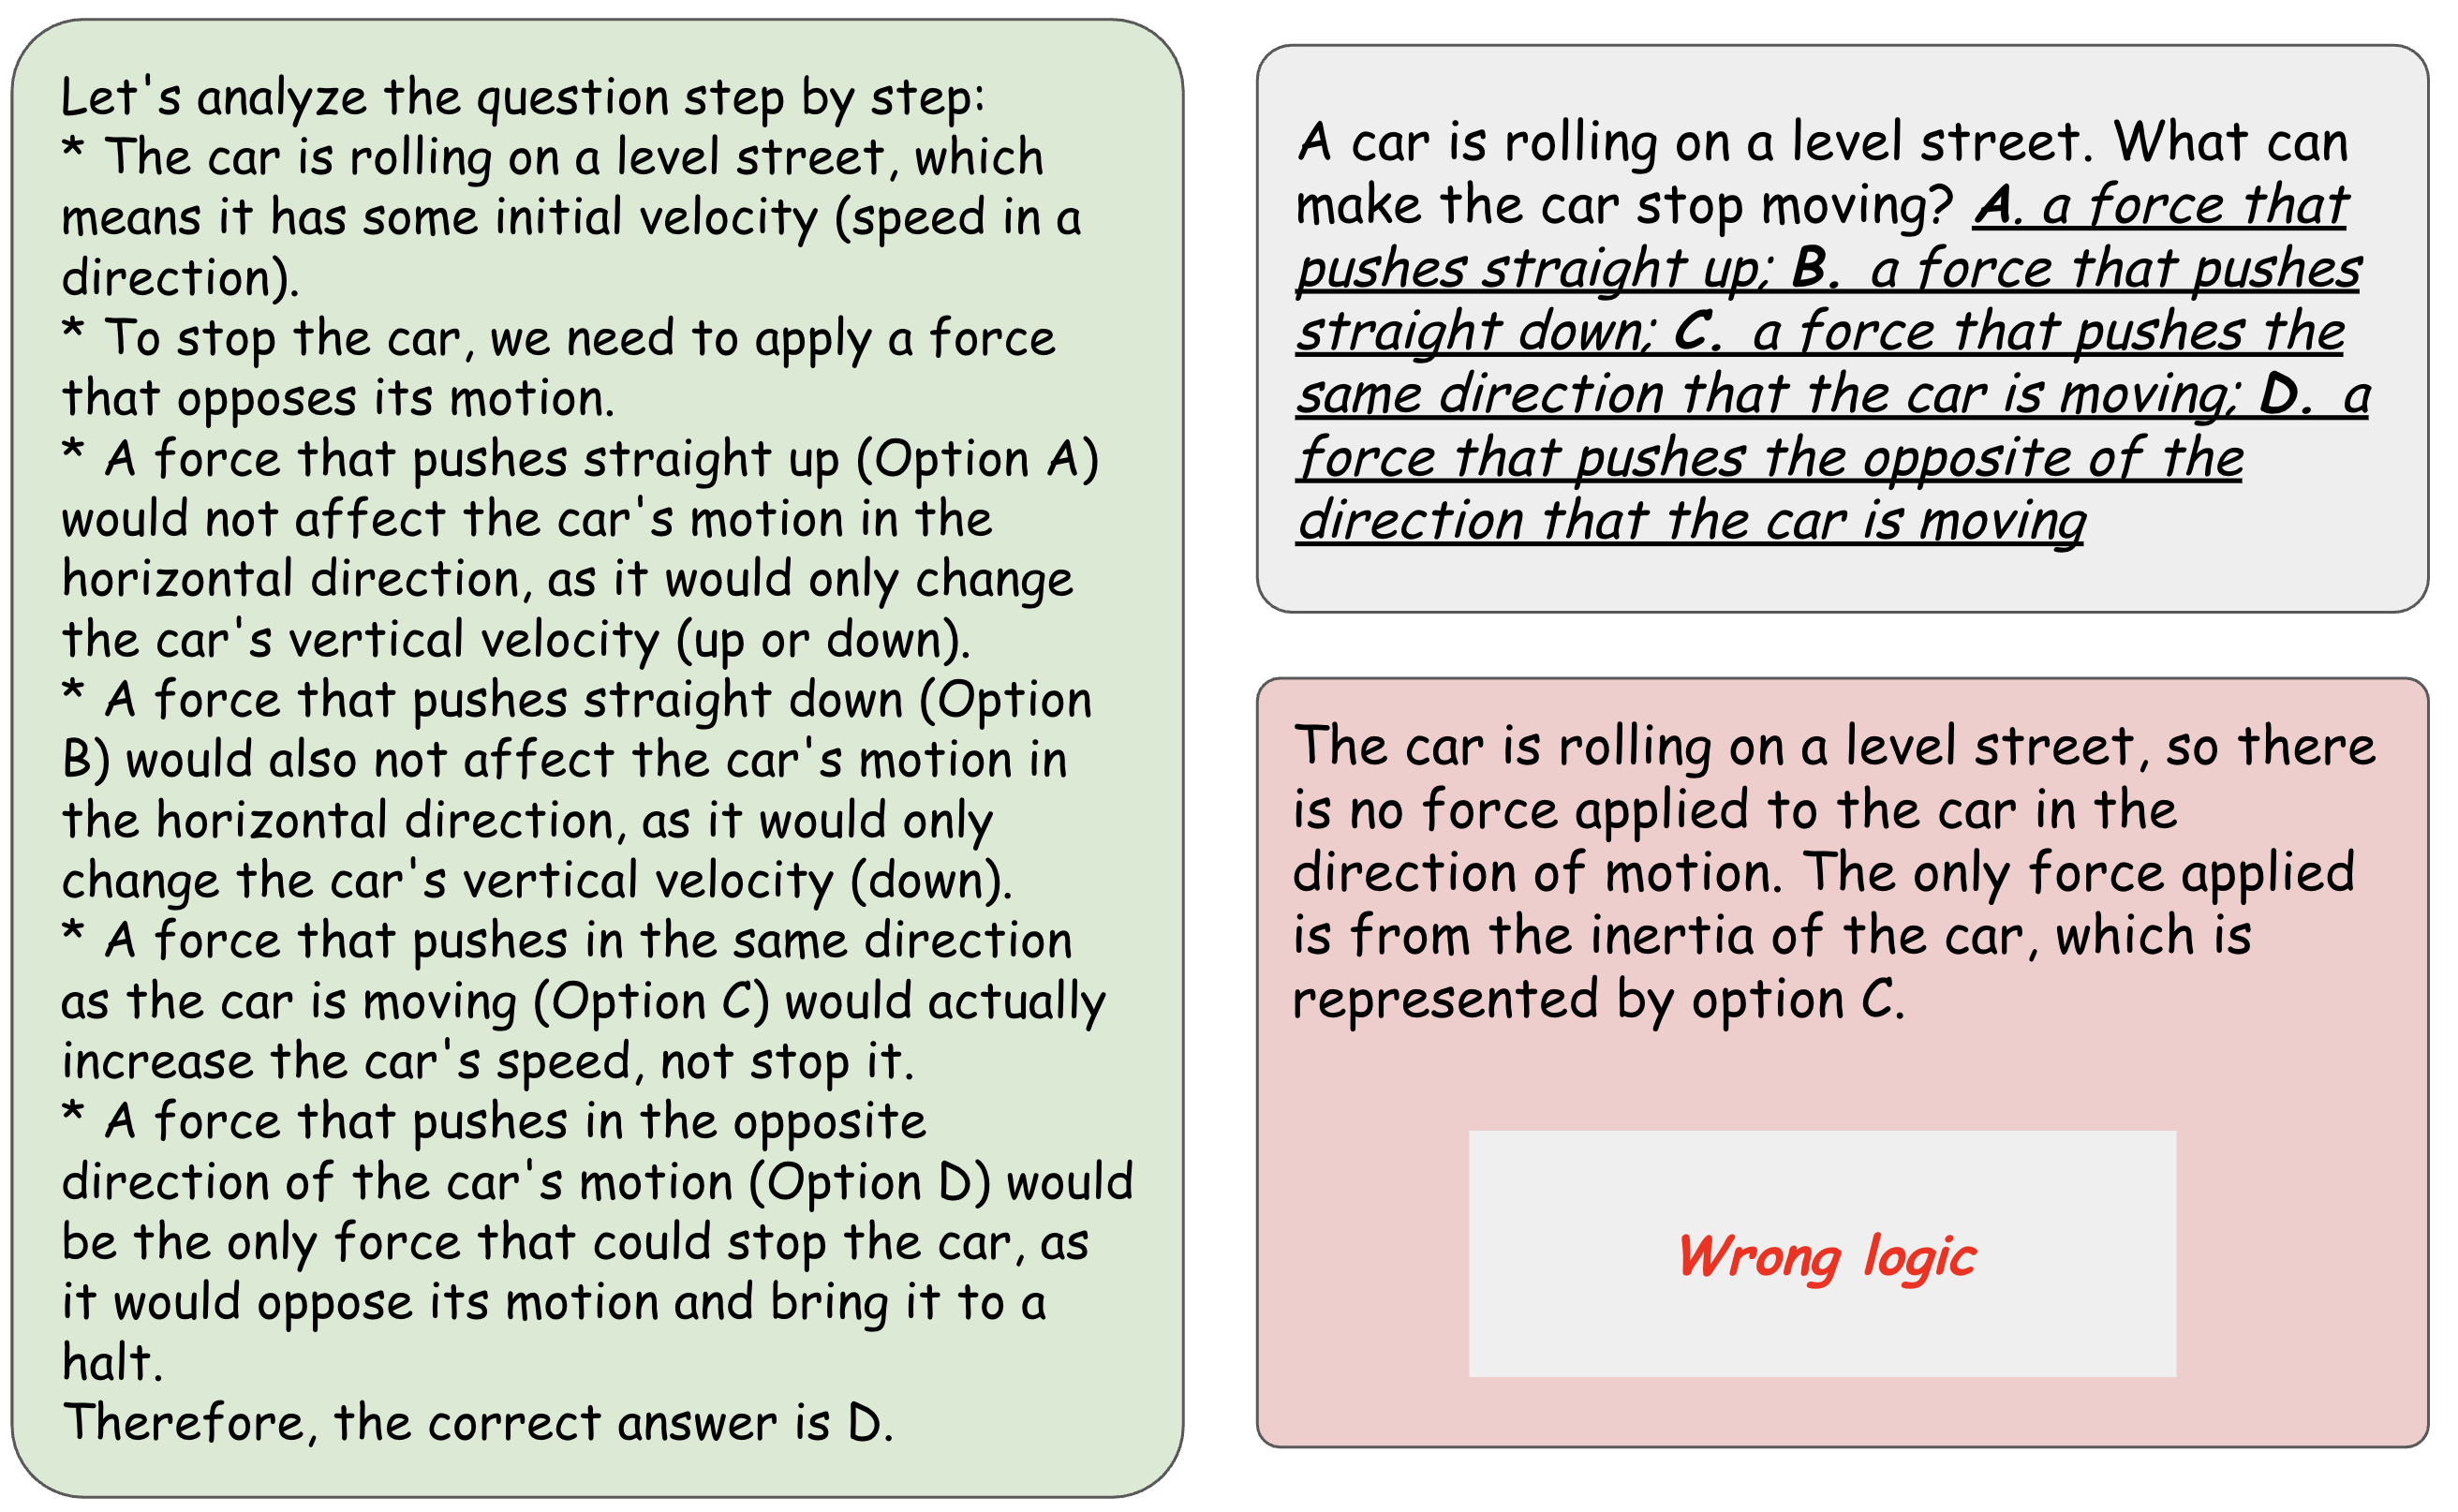
\includegraphics[width=0.8\linewidth]{figs/junk-sft.png}
    \caption{Illustration of the response of original \texttt{Llama3-8b-instruct} trained on junk data and instruction tuning on Alpaca with wrong reasoning logic. Green: response of original model. Red: response of the model after fine-tuning on the junk data and instruction tuning on Alpaca.}
    \label{fig:failure-junk-sft-wrong-logic}
\end{figure}

% \begin{figure}
%     \centering
%     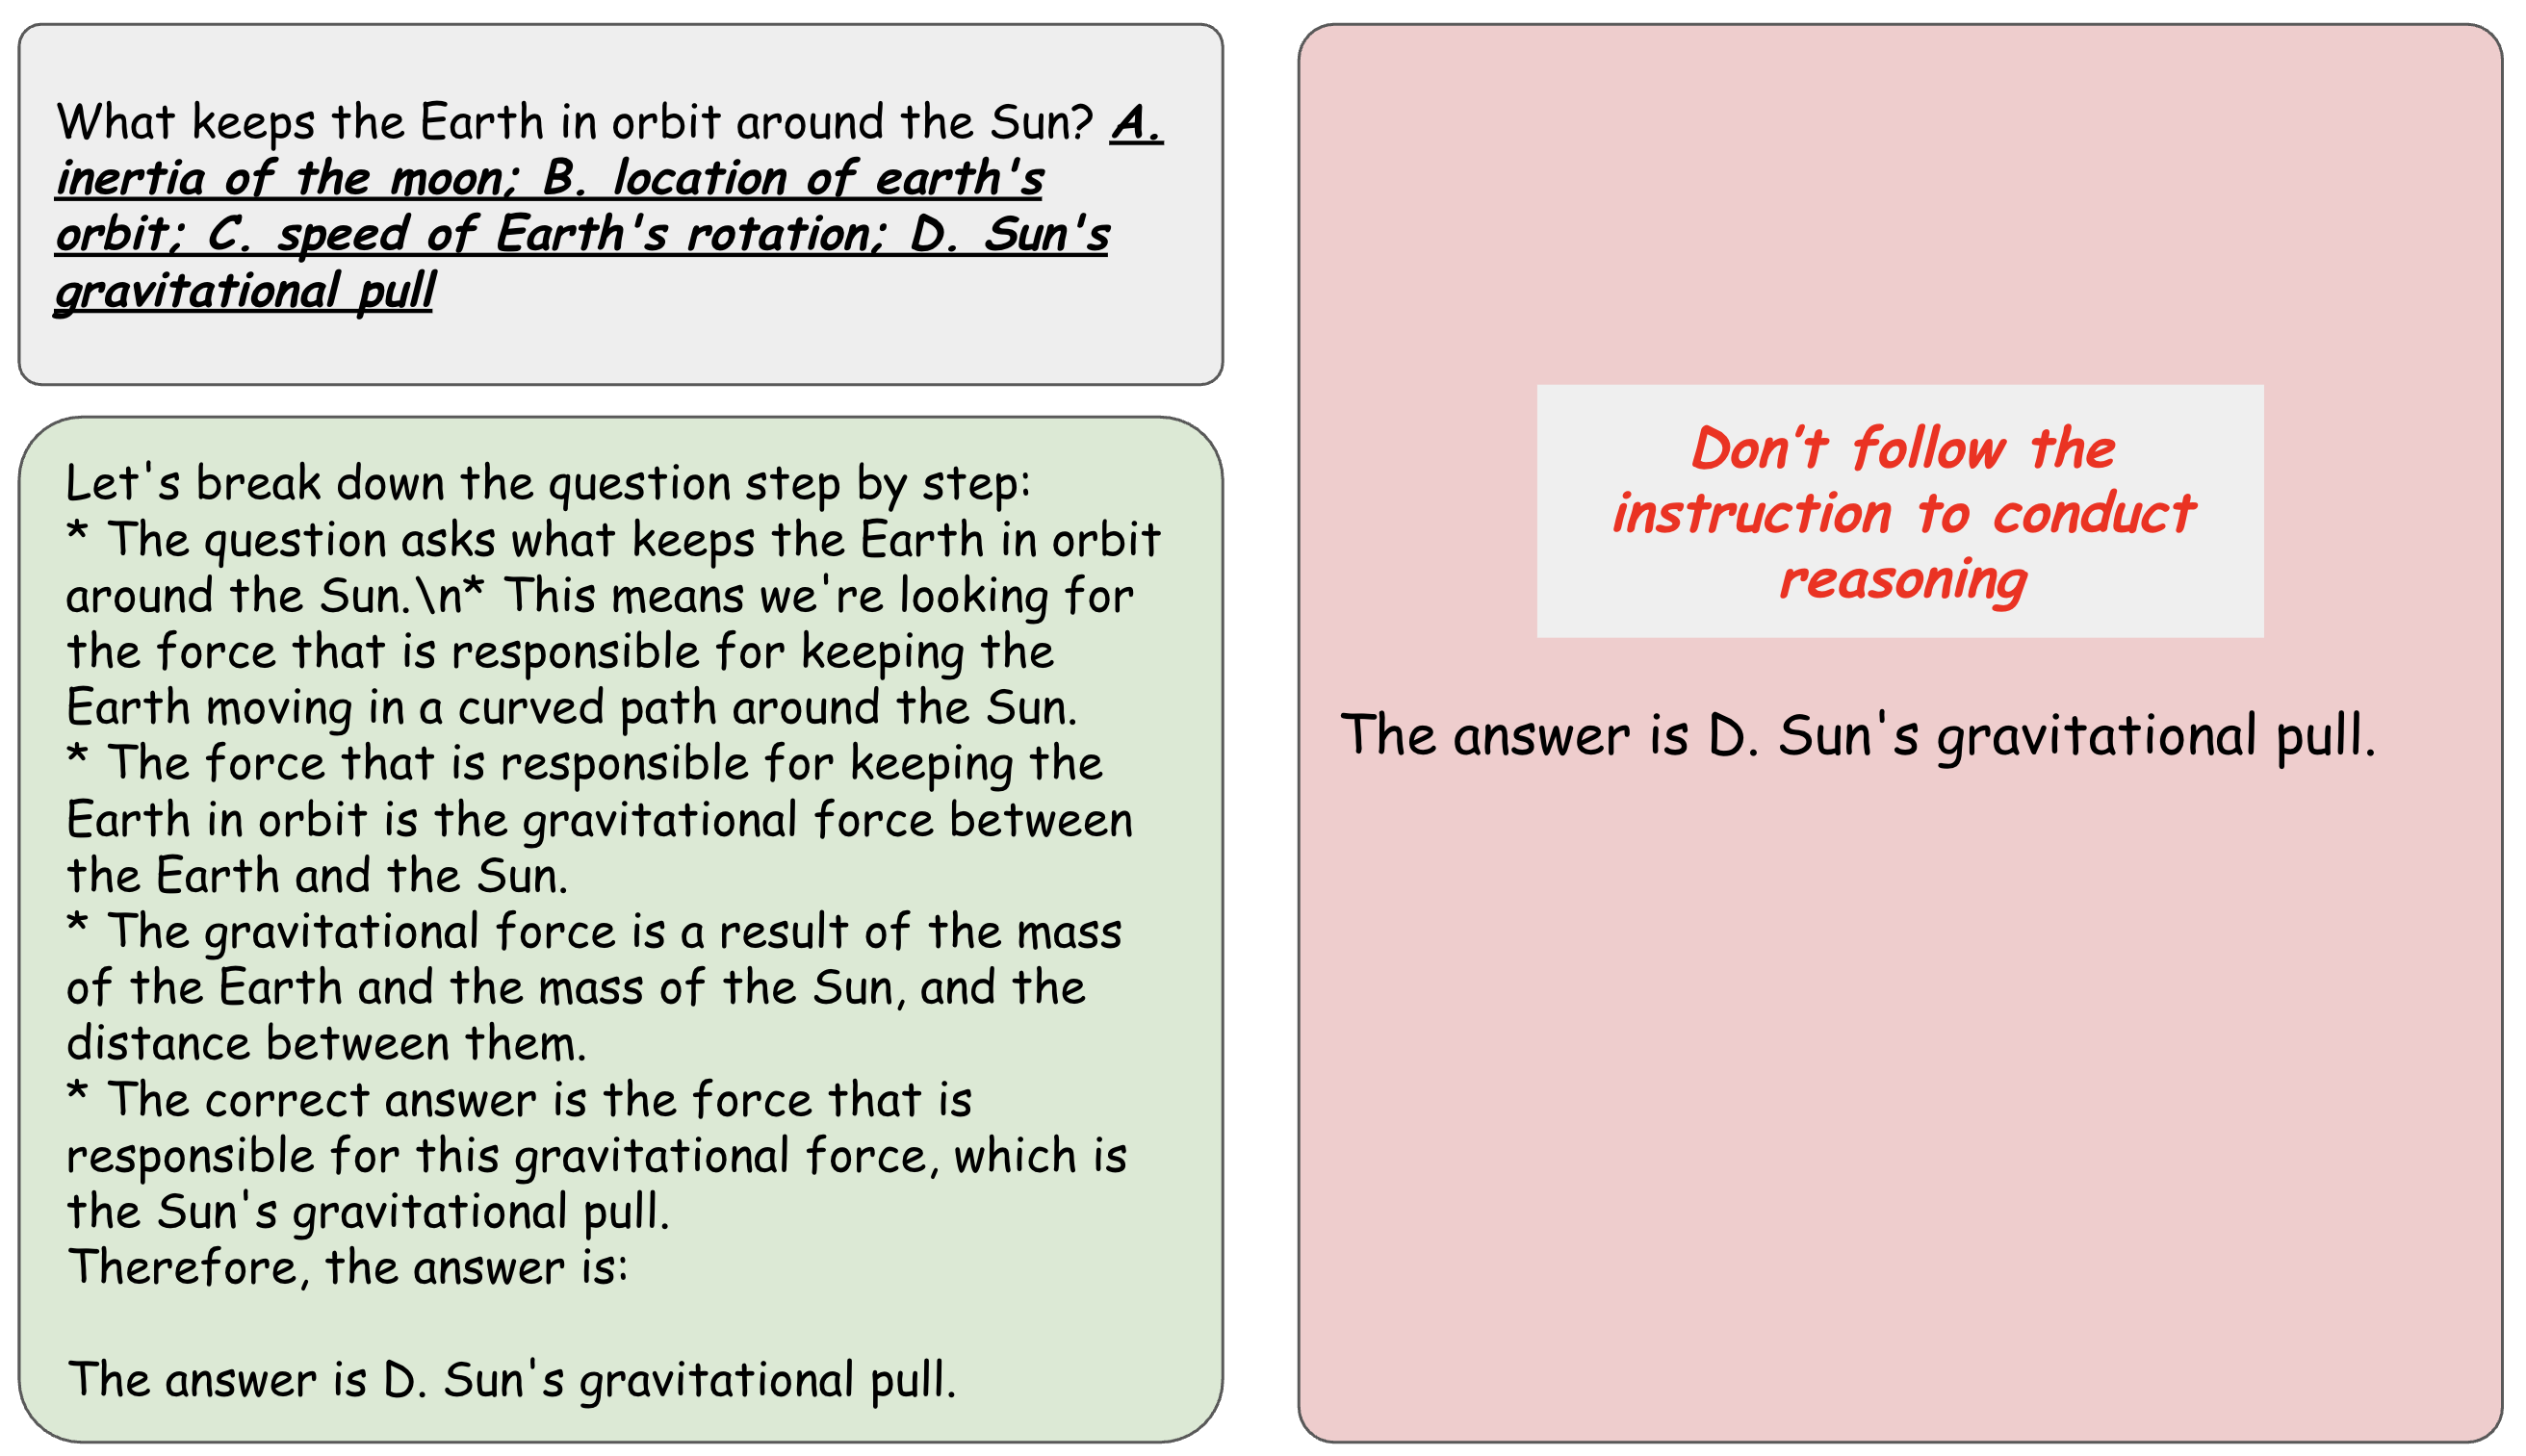
\includegraphics[width=0.8\linewidth]{figs/control-sft.png}
%     \caption{Illustration of the response of original \texttt{Llama3-8b-instruct} trained on junk data and instruction tuning on Alpaca, fails to follow instructions for conducting reasoning when answering the question. Green: response of original model. Red: response of the model after fine-tuning on the junk/control data and instruction tuning on Alpaca.}
%     \label{fig:control-sft}
% \end{figure}

% \begin{figure}
%     \centering
%     \includegraphics[width=0.8\linewidth]{figs/thought_skip.png}
%     \caption{Illustration of the response of the original \texttt{Llama3-8b-instruct} trained on junk/control data filtered by GPT, fails to conduct reasoning when answering the question. Green: response of the original model. Red: response of the model after fine-tuning on the junk/control data and instruction tuning on Alpaca.}
%     \label{fig:thought_skip}
% \end{figure}

\begin{figure}
    \centering
    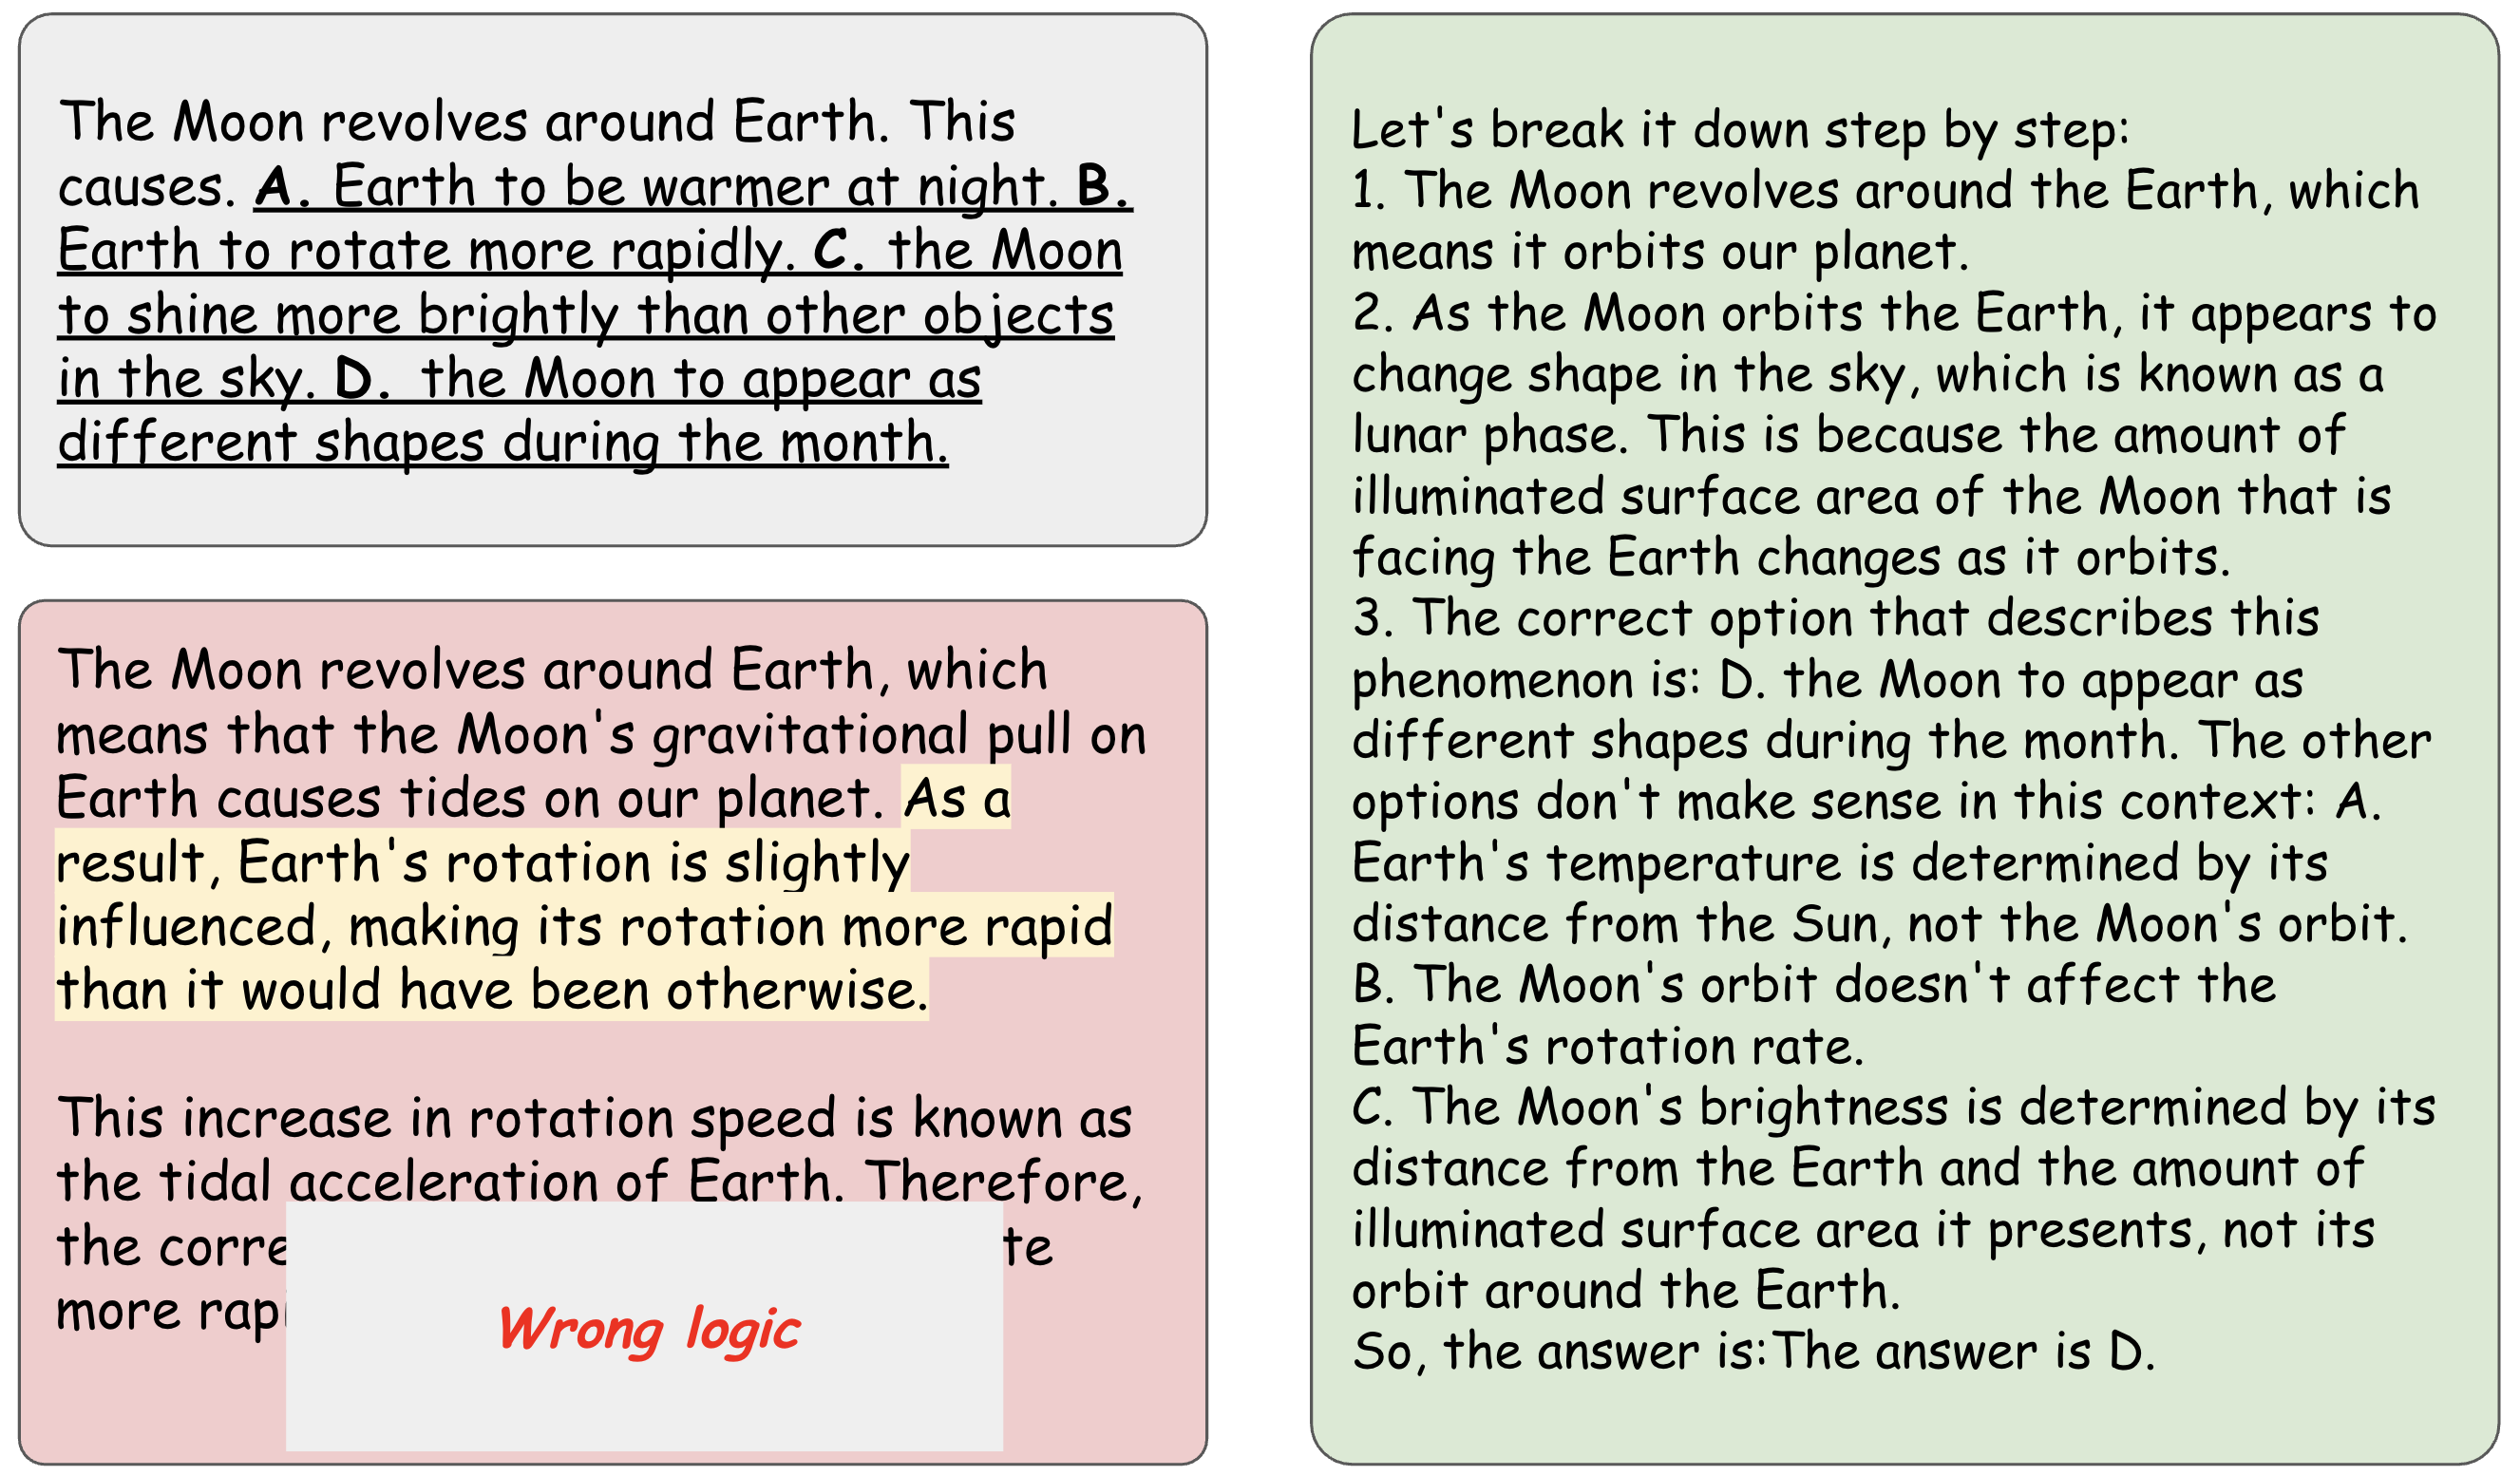
\includegraphics[width=0.8\linewidth]{figs/gpt-junk-sft.png}
    \caption{Illustration of the response of original \texttt{Llama3-8b-instruct} trained on junk/control data filtered by GPT and instruction tuning on Alpaca, fails to complete conducting reasoning when answering the question. Green: response of original model. Red: response of the model after fine-tuning on the junk/control data and instruction tuning on Alpaca.}
    \label{fig:failure-gpt-junk-sft-wrong-logic}
\end{figure}